\chapter{Implementation}

In this chapter, we will illustrate our {\em AngrDBG} library, a debugger-agnostic implementation of the technique described in Chapter 2 based on the binary analysis framework {\em angr}. We will present also two frontends based on that library, one for the {\em GNU Debugger}, {\em AngrGDB}, and the other for the {\em IDA Pro} debugger, {\em IDAngr}.

\section{Angr Overview}

{\em Angr} \cite{shoshitaishvili2016state} is more than just a symbolic execution engine but we will focus on this aspect.

A particular feature is that the framework is cross-architecture and cross-platform. Additionally, angr has well documented and extremely easy-to-use first-level APIs.

Angr is written in Python with some C wrappers. This may affect the performance of the engine but most of the analysis techniques are algorithmically slow and so the language performance is not very relevant.

Angr is under constant development and is made up of several modules. We will present only the ones that are relevant to our approach:

\begin{itemize}
\item {\em CLE}, a multi-format binary loader with an easy API;
\item {\em archinfo}, a collection of classes that contain architecture-specific information;
\item {\em PyVEX}, a wrapper around Valgrind's VEX IR lifter \cite{Net:phd2004}, used to make the analyses architecture-agnostic;
\item {\em Claripy}, the angr data backend, a wrapper around the Z3 solver and an interface to abstract concrete and symbolic values handling;
\end{itemize}

The symbolic execution engine is in the main package of angr, as other analyses and utilities like CFG recovery, value-set analysis, and data dependence analysis.

One of the main advantages of angr for our purpose is that everything is like a plugin. In the implementation of our technique, we have changed some low-level bits in angr without the need to fork the project.

\subsection{Fundamental Classes}

According to \cite{angrdoc} the fundamental high-level types of angr are the following:

\subsubsection{Project}

The {\em Project} is the control base in angr. Project creation invokes the CLE loader. With a Project, you are able to initialize a symbolic execution engine or dispatch an analysis.

\subsubsection{BitVec}

A {\em bitvector} is just a sequence of bits. In Angr this is the basic datatype. A bitvector can be concrete or symbolic. Performing operations with bitevectors will yield a tree of operations that are translated into constraints for the SMT solver.

\subsubsection{Loader}

The {\em CLE loader} gets the representation in a virtual address space of a program from a binary file. It solves relocations and loads also the needed libraries. CLE supports many formats and operating systems binaries, including ELF for Linux and PE for Windows.

\subsubsection{SimState}

A {\em SimState} is the representation of the program state inside the symbolic executor. Memory, registers, file system and all data that can change during the execution are in the state.
These entities are organized in plugins and are accessible using the proper field. For example, the memory plugin can be accessed with \verb|state.memory| and the plugin that handles environment interaction on POSIX-compatible systems is accessible with \verb|state.posix|.

Must-know plugins are regs and mem. With \verb|state.regs.<register name>| you can inspect the state registers and with \verb|state.mem[address].<type>| you can inspect the memory, where  \verb|<type>| is a standard type such as the integer types defined inside the {\tt stdint.h} or the string type.

\subsubsection{Simulation Manager}

The {\em simulation manager} is the primary interface to the symbolic execution engine (used for the exploration). It is the way to get the next state from the current.

The exploration can be driven with {\em find} and {\em avoid} conditions. These conditions may be addresses that must be reached in order to terminate the exploration of a path and classify it as valid or not.
They can be also functions that inspect the current state to determinate if the exploration has found a result.

\subsection{Memory Plugin}

The angr memory structure is quite complex and multi-layered. In this section, we present only a very high-level overview. 

The main goal of the memory plugin is to provide an interface for the load and store primitives for both concrete and symbolic values.

First of all, outside the memory plugin, the executable file is loaded and mapped by CLE in a so-called {\em Clemory} object. This is used by the memory plugin as a read-only memory backer to lazily load into the process address space the initial content of the memory for a binary.

The memory plugin follows a page-oriented model.
This is realized through the abstract {\em Page} class, whose default concrete implementation is based on a Python list. A Page instance indexes all objects in the memory space associated with the corresponding page.

Page objects are managed by an instance of the {\em SimPagedMemory} class.
SimPagedMemory loads pages in a lazy way based on the requests to the memory plugin. A Page content is initialized to concrete values if the requested page address is in the range of the associated Clemory object. When the page does not belong to the Clemory object (e.g. a stack page) it is left uninitialized to make a request return an unconstrained symbolic value.

The high-level class that represents the process memory space is {\em SimMemory}. The load/store requests are mapped to the paged memory keeping also a record for symbolic memory addresses. 

In VEX, the intermediate representation used by angr, registers are mapped to a separate memory, so a SimMemory is used also with registers operations.

\subsection{Simprocedures}

A {\em SimProcedure} is used to define a hook in angr. Simprocedures are mainly used with external functions hooking the associated symbol. In this way angr can skip the exploration of known library functions.

A SimProcedure is essentially a model of the function behavior written with the aim of minimizing the number of forks generated by the SimProcedure itself.

\section{AngrDBG}

{\em AngrDBG} is the library that we developed to synchronize a concrete process state with an angr state.

angr, as we said in the previous section, is composed of plugins and AngrDBG exploits this feature to modify parts of angr.

The fundamental function exposed to the user is {\em StateShot}. StateShot initializes an angr state with the current debugger context and changes the memory plugin of the state with a custom version.
The memory plugin is responsible for requesting concrete memory from the debugger when the engine wants to access a memory region mapped in the process.

A state returned by StateShot can be used like any other angr state.

The project is a global instance created lazily with \verb|load_project| that uses the same image base of the debugged process.

\subsection{Abstract Debugger}

We designed this library to be debugger independent using an abstraction layer. So AngrDBG is compatible with various tools that have Python bindings.

{\em Debugger} is the virtual class that makes this possible. Any tool that wants to synchronize angr with a specific debugger needs to implement a subclass of the Debugger class.
The global \verb|register_debugger(debugger)| routine must be invoked to tell AngrDBG to use a specified instance of a Debugger subclass as the source of data for the synchronization.

\verb|get_debugger| is used to get the currently registered instance.

The methods that must be implemented are the following:

\begin{itemize}
\item \verb|before_stateshot(self)| An event handler triggered before the synchronization setup in StateShot, just after the empty state creation;
\item \verb|after_stateshot(self, state)| An event handler triggered before the StateShot return;
\item \verb|is_active(self)| Return True if the debugger is running the target process;
\item \verb|input_file(self)| Return a Python file-like object of the target executable;
\item \verb|image_base(self)| Return the process base address;
\item \lstinline{get_<byte|word|dword|qword>(self, addr)} Read an byte|word|dword|qword from the memory as a Python int (4 distinct methods). The endianness must be concordant with the debugged process architecture;
\item \verb|get_bytes(self, addr, size)| Read a string from the memory;
\item \lstinline{put_<byte|word|dword|qword>(self, addr, value)} Write a Python int as a byte|word|dword|qword to memory (4 distinct methods). The endianness must be concordant with the debugged process architecture;
\item \verb|put_bytes(self, addr, value)| Write a string to memory;
\item \verb|get_reg(self, name)| Get a register value;
\item \verb|set_reg(self, name, value)| Set a register value;
\item \verb|step_into(self)| Call the debugger "step into" command;
\item \verb|run(self)| Run the process inside the debugger;
\item \verb|wait_ready(self)| Wait until the debugged process is ready to be inspected;
\item \verb|refresh_memory(self)| Refresh the information about the memory space inside the debugger. This is needed when the debugger uses a cache for this information;
\item \verb|seg_by_name(self, name)| Get a Segment object by the name;
\item \verb|seg_by_addr(self, name)| Get a Segment object by the address;
\item \verb|get_got(self)| Get a tuple (start address, end address) related to the GOT section when using the ELF file format;
\item \verb|get_plt(self)| Get a tuple (start address, end address) related to the PLT section when using the ELF file format;
\item \verb|resolve_name(self, name)| Resolve a symbol to its address using the name;
\end{itemize}

\subsection{Memory Synchronization Types}
\label{angrdbg_memtypes}

In AngrDBG a user can choose between four different types of memory synchronization.

The related functions are \verb|get_memory_type()| and \verb|set_memory_type(mem_type)| where \verb|mem_type| is one of the following constants:

\subsubsection{SIMPROCS\_FROM\_CLE}

The concrete memory is from the target process but, when using the ELF file format, the SimProcedures are maintained as in a regular empty angr state generated using CLE data. This is done to avoid the execution of library code but at the same time support self-modifying code. When an external function does not have a SimProcedure, the symbol is resolved and the GOT section is populated with the real address to avoid the exploration of the loader code.

The PE format is not currently supported by this type of memory synchronization.

\subsubsection{ONLY\_GOT\_FROM\_CLE}

Like the previous one, but with a SimProcedure stub that returns an unconstrained symbolic value used to model unknown imported functions.

The PE format is not currently supported by this type of memory synchronization.

\subsubsection{USE\_CLE\_MEMORY}

The segments associated with the executable file are borrowed from the CLE loader and only the segments created at runtime, like the stack, are from the concrete process. This is not accurate if the program modified some variables in .data or if it has a self-modifying code.

\subsubsection{GET\_ALL\_DISCARD\_CLE}

All the memory is from the target process, on ELFs should be used only with \verb|LD_BIND_NOW| to avoid the exploration of loader code. This should be the preferred option on Windows at the moment.

\subsection{Memory Plugin}

To synchronize the memory we extended the memory plugin to load values from the debugged process.

The replacement of the Page class is {\em DbgPage}. It is a list of bytes that works lazily. When a load request occurs, the requested data is returned if it is in the list, otherwise, if the \verb|from_dbg| attribute is present in the DbgPage object the correspondent bytes are requested to the debugger. Without the \verb|from_dbg| attribute, so when the page does not belong to the concrete address space, an unconstrained symbolic value is returned.

{\em SimDbgMemory} is the correspondent class to SimPagedMemory. We patched the page initialization method. If the memory type is \verb|USE_CLE_MEMORY| and the requested page is in the Clemory backer it loads the page from the backer like angr usually does. In the other situations the page is initialized as empty (remember that DbgPage works lazily) and the permissions are got from the debugger when possible.

{\em SimSymbolicDbgMemory} is the high-level class, simply a version of SimMemory that works with SimDbgMemory instead of SimPagedMemory.

In the StateShot routine, the state is created specifying SimSymbolicDbgMemory as the memory plugin.

\subsection{Internal process state synchronization}

We implemented the retrieval of the relevant process related values in the operating system executing syscalls on-the-fly.

The method is the following:

\begin{itemize}
\item Save the context of the concrete process and the first bytes of the executable segment;
\item Write the syscall instruction (int 80h on x86) at the beginning of the executable segment;
\item Set input registers and the program counter to the syscall instruction address;
\item Execute the syscall with a single step in the debugger;
\item Retrieve the results;
\item Restore the context and the previously patched bytes;
\end{itemize}

%The syscall instruction (int 80h on x86) is written at the beginning of the executable segment, then the context is saved and the target syscall is executed.

The current implementation supports the retrieving of the BRK\footnote{The top of the Heap segment} value.

File and network operations return by default symbolic values. Reading from a file descriptor gives uninitialized symbolic memory. A custom behavior (e.g. load concrete data from a file in the disk) can be forced by creating an \verb|angr.SimFile| object and linking it to the initial state, as explained in \cite{angr_file_doc}.

Segment registers are missing from the synchronization. At the moment all memory read using a segment register (like the stack canary) is symbolic.

\section{Using AngrDBG API}

AngrDBG comes with a wrapper class around StateShot, {\em StateManager}, that allows the user to easily create a state from the debugger state and manage the symbolic values creation and concretization. This class is also responsible to keep track of the symbolic inputs and inject them into the debugger after the exploration.

The exposed methods are the following:

\begin{itemize}
\item \verb|sim(self, key, size=None)| Set a value as symbolic. Key can be an address (int) or a register name (string). If the size parameter is not specified it is the default register size when the key is a register or the size of a pointer in the debugged program architecture when the key is an address.
\item \verb|__getitem__(self, key)| The get operator. If the key is a register name return the associated value. If the key is an address access to the state memory in the same way of angr with \verb|state.mem|.
\item \verb|__setitem__(self, key, value)| The set operator. If the key is a register name overwrite the register content. If the key is an address write to the state memory in the same way of angr with \verb|state.mem|.
\item \verb|simulation_manager(self)| Load the global project and generate a simulation manager based on the current state.
\item \verb|to_dbg(self, found_state)| Concretize the corresponding symbolic values in \verb|found_state| and write that values in the debugger. \verb|found_state| can be an angr state or another StateManager instance.
\item \verb|concretize(self, found_state)| Like \verb|to_dbg| but return the concretized value in a dictionary instead of writing the values to the debugger.
\end{itemize}

\subsection{Remote Server}

Angr explorations require a huge amount of RAM. To allow the usage of angr in a powerful hardware setup and improve the exploration time AngrDBG and the debugger can run in different machines.

The command \verb|python -m angrdbg| starts an rpyc \cite{rpyc} based server. The default host is localhost in order not to expose an unsecure connection. The user must do SSH port forwarding to set up a secure connection.

The angrdbg server waits for two rpyc connections and after that, it opens an IPython \cite{ipython} kernel in the current TTY. The first connection is used to serve data to the IPython shell, so the roles of client-server are swapped in this case. The second is used to wait for remote procedure calls from the client.

The two connection lives in different processes to avoid race conditions.

% insert diagram here


\section{AngrGDB}

{\em AngrGDB} is in its core an implementation of the Debugger class of AngrDBG using the GDB Python bindings.

It works also with remote debugging sessions so you can, for example, attach GDB to QEMU and perform symbolic execution using AngrGDB.

The methods \cite{gdb_py_doc} that are invoked to retrieve information are gdb.execute, used to execute a GDB command (e.g. "info address"), \verb|write_memory| and \verb|read_memory|.

\subsection{Using AngrGDB}

To use AngrGDB you can simply open a Python shell under GDB (with the "pi" command) and use the AngrDBG API.

In addition, we defined some custom GDB commands to easily explore code using find and avoid targets.

The commands are the following:

\begin{code}
angrgdb sim <register name> [size]
angrgdb sim <expression> [size]
\end{code}
Set a memory/register as symbolic

\begin{code}
angrgdb list
\end{code}
List all items that you setted as symbolic

\begin{code}
angrgdb find <address0> <address1> ... <addressN>
\end{code}
Set the list of find targets

\begin{code}
angrgdb avoid <address0> <address1> ... <addressN>
\end{code}
Set the list of avoid targets

\begin{code}
angrgdb reset
\end{code}
Reset the context (symbolic values and targets)

\begin{code}
angrgdb run
\end{code}
Generate a state from the debugger state and run the exploration

\begin{code}
angrgdb shell
\end{code}
Open an IPython shell with a StateManager instance created from the current GDB state called "sm"

\section{IDAngr}

{\em IDAngr} is not simply an AngrDBG frontend library for the IDA Pro \cite{ida} debugger but it has also a graphical interface in Qt integrated directly in IDA.

It can be loaded using the "load script" command in the File menu or installed as a plugin and invoked using the Ctrl-Alt-I keyboard shortcut.

IDAngr implements also the remote AngrDBG protocol and can be attached to a remote AngrDBG server, as explained in section 3.3.1.

Before to use the AngrDBG API the library must be initialized.

The first method that must be called is \verb|idangr.init|. Without specifying arguments, the AngrDBG and Angr modules will be imported using the regular python import statement and the exploration will be performed in the same machine running IDA Pro. If the host and port arguments are present the selected remote AngrDBG server will be connected to IDAngr.

\subsection{GUI Overview}

The initialization process can be done also using the GUI. When the plugin is called for the first time a popup window asks the user if he wants to initialize a local or a remote AngrDBG instance.

The graphical components added to IDA are two: a context menu entry in the menu shown when clicking the right button of the mouse and a panel inserted alongside the IDA View.

In the context menu, Figure \ref{fig:ctx_menu}, you can perform the following actions:

\begin{itemize}
\item {\em Find}: add the current selected address to the simulation manager's find targets;
\item {\em Avoid}: add the current selected address to the simulation manager's avoid targets;
\item {\em Symbolic}: symbolize a memory region starting from the current selected address and specifying its size, Figure \ref{fig:add_symbolic};
\end{itemize}

\begin{figure}
    \centering
    \parbox{5cm}{
        \caption{The context menu.}
        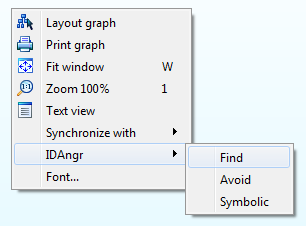
\includegraphics[width=5cm]{ctx_menu}
        \label{fig:ctx_menu}
    }
    \qquad
    \begin{minipage}{5cm}
    \caption{The Add symbolic memory prompt.}
    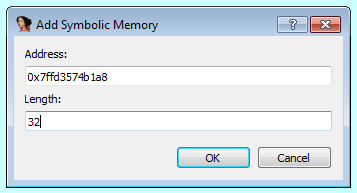
\includegraphics[width=5cm]{add_symbolic}
    \label{fig:add_symbolic}
    \end{minipage}
\end{figure}

The IDAngr panel is the core graphical component of the plugin. In the panel, you can view the values selected using the context menu. You can also set symbolic registers, as in Figure \ref{fig:panel1}.

By right-clicking on a row of the symbolic memory or registers views you can set the preconditions using python (figure \ref{fig:precond}), jump to its address in the IDA view or remove it.

By right-clicking on a row of the find or avoid view you can jump to its value or delete it.

The buttons at the top of the panel are the following:

\begin{itemize}
\item {\em RESET}: Delete all symbolic values and find/avoid targets
\item {\em RUN}: Show the exploration prompt, Figure \ref{fig:run}, in order to start the symbolic exploration
\item {\em NEXT}: Show the exploration prompt, Figure \ref{fig:run}, in order to reach another valid state after a previous exploration
\item {\em TO DBG}: Use a valid found state to concretize all symbolic values listed in the panel and inject them in the debugger
\item {\em View File Dump}: Use a valid found state to dump the content of a file using its file descriptor
\end{itemize}

The exploration prompt is the last step left to the user before the symbolic exploration. This window allows you to set which memory type use (based on Section \ref{angrdbg_memtypes}) and set a python function as find or avoid condition instead of using the list of targets in the panel.

The correspondent types of memory synchronization:

\begin{itemize}
\item \verb|SIMPROCS_FROM_CLE|: use simprocs in got when possible
\item \verb|ONLY_GOT_FROM_CLE|: get entire .got from CLE (with stubs)
\item \verb|USE_CLE_MEMORY|: get binary memory from CLE
\item \verb|GET_ALL_DISCARD_CLE|: full debugger memory
\end{itemize}

Hooks are at the moment not supported in the graphical interface, but they can be used from IDAPython as regular angr hooks. Simply use \verb|load_project| to get the current project and apply hooks on it:

\begin{py_code}
p = angrdbg.load_project()
@p.hook(0xdeadbeef)
def hook(state):
    print "I'm at", state.regs.rip
\end{py_code}

\begin{figure}[H]
  \caption{The symbolic values and the find/avoid lists in the panel.}
  \centering
  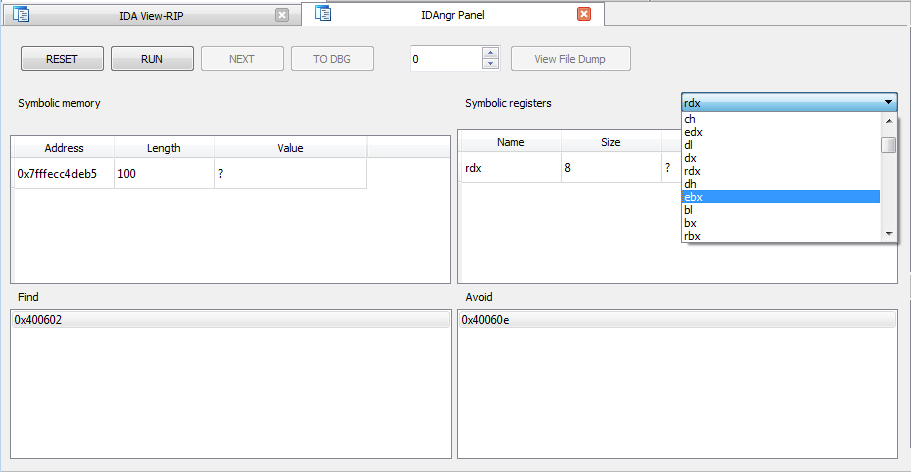
\includegraphics[width=1\textwidth]{panel1}
  \label{fig:panel1}
\end{figure}
\begin{figure}[H]
  \caption{Setting preconditions on a symbolic value.}
  \centering
  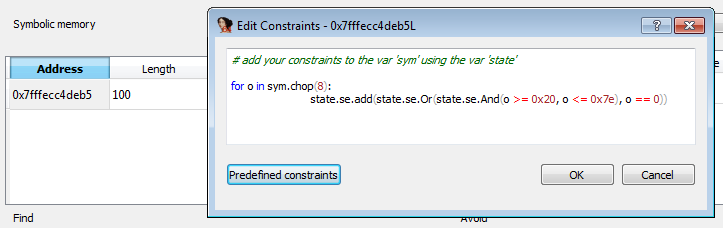
\includegraphics[width=0.8\textwidth]{precond}
  \label{fig:precond}
\end{figure}
\begin{figure}[H]
  \caption{The exploration prompt.}
  \centering
  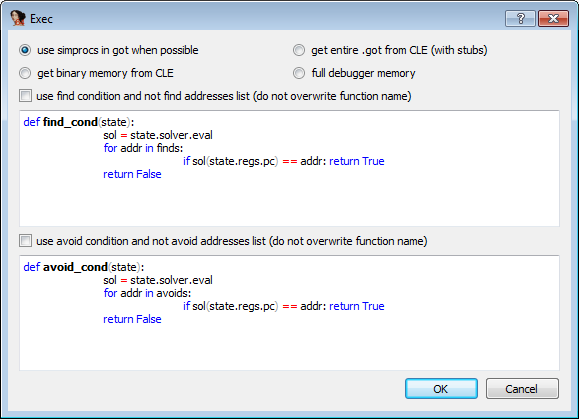
\includegraphics[width=0.6\textwidth]{run}
  \label{fig:run}
\end{figure}

